
\section{Experimentation}

In this experimental part we study the numerical stability and limit of the method considing toy benchmark problems. Supervised learning is targeted since it is a direct way to evaluate the method efficiency and robustness. Let us remember that we do not evaluate learning performances here, only the way we can adjust recurrent network weights.

\subsection*{Software implementation}

In order to provide so called reproducible science \cite{topalidou_long_2015}, the code is implemented as a simple, highly modular, fully documented, open source, object oriented, easily forkable, self contained, middle-ware, and is available here: 
\\\centerline{\href{https://vthierry.github.io/mnemonas}{https://vthierry.github.io/mnemonas}.}\\ 
A minimal set of standard mechanisms (random number generation, histogram estimation, linear system resolution, system calls) is used. The main part of the implementation hierarchy is show in Fig.~\ref{class-hierarchy}. 

\begin{figure}[!ht]
  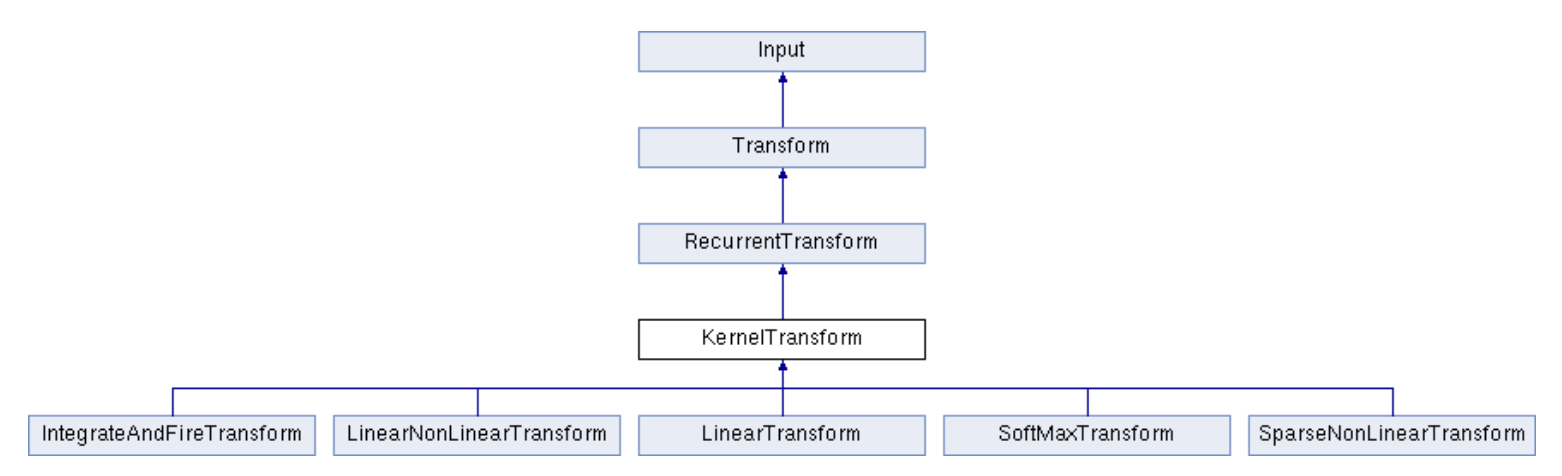
\includegraphics[width=\textwidth]{img/class-hierarchy}
  \caption{A view of the class-hierarchy: A {\tt Input} simply provides a $x_n(t), n \in \{0, N\{, t \in \{0, T\{$ values, while a {\tt Transform} provides such values given another {\tt Input}, while other objects defined here derive from such an oversimple abstract class, and are precisely defined and discussed in Appendix~\ref{generality}.}
  \label{class-hierarchy}
\end{figure}

Regarding the estimations described in Appendix~\ref{application}, the {\tt KernelSupervisedEstimator} class implements, quadratic estimation, bounded and unbounded robust estimation and Boolean estimation, while the {\tt KernelObservableEstimator} class implements some basic stochastic models estimation.

For run-time performances and inter-operability with different programming languages a {\tt C/C++} implementation (with the compilation scripts) is proposed, the wrapping to other programming languages (e.g., {\tt Python}, available in the present implementation) being straightforward, using e.g. {\tt swig}. 

The first experimental verification is that it is quite simple to define the main unit structures in Appendix section~\ref{generality} from {\tt KernelTransform} as claimed in the paper, see Fig~\ref{AIF-kernel-implementation} for an example with AIF nodes and the code source for the LNL {\tt LinearNonLinearTransform} implementation and the SoftMax {\tt SoftMaxTransform} implementation.

\begin{figure}[!ht]
  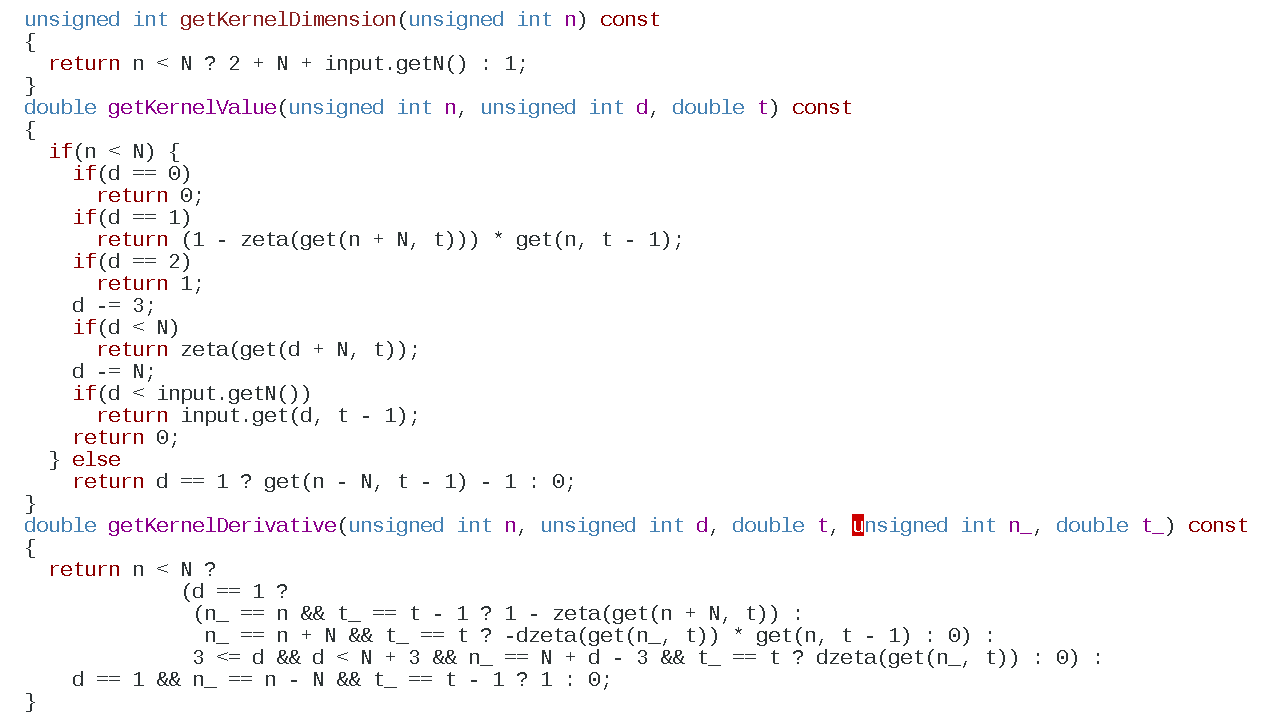
\includegraphics[width=\textwidth]{img/AIF-kernel-implementation}
  \caption{The implementation of the AIF node, translating equation~(\ref{st-lnl-network}) into the notation of equation~(\ref{eq-recurrent}) in the {\tt IntegrateAndFireTransform} object.}
  \label{AIF-kernel-implementation}
\end{figure}

\subsection*{Using reverse engineering}

As being in a deterministic context, we are going to rely on a reverse engineering setup, in order to evaluate the performances and limit of the method. An input/output learning sequence is going to be generated by a input/output {\em root} network of $\bar{N}$ units and another {\em learning} network with random initialization is going to re-estimate the transform. This guaranties the existence of an exact solution. 

How relevant is it to use such a reverse engineering setup ? On one hand, surprisingly enough perhaps, such networks (at least deep networks \cite{Zhang2016Understanding}) behave with the same order of magnitude of performances, the input being either ``meaningful'' or not, in the sense it represents data with a semantic or not. We thus can expect simple random input/output tests to be relevant estimation of performance, even for more semantic application. On the other hand, as developed in Appendix~\ref{closedforms}, several ``challenging'' tests are in fact highly dependent on the chosen architecture, with often trivial solution, as soon as the hidden architecture is well chosen. The key point is thus to see if several kind of nodes can be adjusted with this mechanism. For these reasons we have considered the reverse engineering paradigm as a first test.

In most of the cases, they are several solutions (e.g.,  in a linear case, up to a permutation of the units, or some linear combination). We consider a root network of $\bar{N}$ units for a sequence of time $T$, for a $M=1$ scalar random input, considering either L (for linear), LNL, AIF or SoftMax units, with random weights (drawn from a Gaussian distribution with $0$ mean and $\sigma \simeq 1/N$ standard deviation, which is know to guaranty a stable non-trivial dynamic). Only the unit of index $n=0$ is considered as output units, i.e., $N_0 = 1$, the $N-1$ remainder units activity being hidden to the estimation. This choice is related to the fact that the adjustment of the hidden units weights is the key challenge.

In this deterministic case, we observe the following parameters: number of steps to convergence, final precision criterion value, and we also fit an exponential decay curve\footnote{{\bf Exponential decay fit.} The criterion value model to fit is of the form: 
\eqline{c(t) \deq \alpha \, e^{-t/\tau} + \beta.}
The time decay $\tau$ is fitted in the least-square sense on $\log(c(t) - c(t-1)) = k - t / \tau$, for $k\deq \log(\alpha\,(1-e^{1/\tau}))$ and the bias $\beta$ is fitted, given $\tau$, on $c(t) = (c(t) - c(t-1))/(e^\frac{1}{\tau}-1) + \beta$. More precisely, the least-square problems write: 
\eqline{\min_{1/\tau, k} \sum_{t}^T \gamma^{T-t} \, (k - t / \tau - \log(c(t) - c(t-1)))^2,}
for an exponential window of width $W=\frac{\log(1 - r)}{\log(\gamma)}$ where $r$ is the fraction of data average within this window (typically 90\%), while the bias is estimated minimizing:  
\eqline{\min_{\beta} \sum_{t=1}^T \, \delta_{0 < \hat{\beta}(t) < \min_t c(t)} \, \gamma^{T-t} \, (\beta - \hat{\beta}(t))^2, \;\;\; \hat{\beta}(t) \stackrel{\rm def}{=} c(t) - \frac{c(t-1) - c(t)}{e^\frac{1}{\tau}-1},}
selecting only minimal values in order to guaranty a coherent estimation of this bias.} in order to estimate the decay time-constant and final criterion bias.

Examples of results for different kind of units are reported in Fig.~\ref{reverse-engineering}, and two typical criterion decay curves are shown in Fig.\ref{criterion-decay-curve}. 

\begin{figure}[!ht]
  \begin{center}{\small
    \begin{tabular}{l|cccccc|}
Node type & \multicolumn{6}{c}{LinearNonLinearTransform} \\
\hline
Number of units & 2 & 4 & 8 & 16 & 32 & 64 \\
Number of Iterations & 36 & 101 & 78 & 101 & 55 & 101 \\
Minimal criterion value & 9.3e-07 & 3.0e-06 & 1.0e-06 &  1.6e-06 & 9.1e-06 & 4.5e-06 \\
Exponential decay time & 24 & 23 & 88 &  37 &  20 &  98 \\
Final bias interpolation & 2.2e-08 & 2.6e-06 & 5.9e-07 & 1.6e-06 & 2.6e-06 & 4.5e-06 \\
\hline
\end{tabular}
 \\
    ~\\
    \begin{tabular}{l|cccccc|}
Node type & \multicolumn{6}{c}{IntegrateAndFireTransform} \\
\hline
Number of units & 2 & 4 & 8 & 16 & 32 & 64 \\
Number of Iterations & 101 & 101 & 101 & 101 & 101 & 101 \\
Minimal criterion value & 9.9e-06 & 4.7e-06 & 1.1e-06 &  3.5e-06 & 7.8e-06 & 1.4e-06 \\
Exponential decay time & 8 & 36 & 17 &  34 & 56 & 23 \\
Final bias interpolation & 9.1e-06 & 4.6e-06 & 1.1e-06 &  3.7e-06 & 7.9e-06 & 1.2e-06 \\
\hline
\end{tabular}
 \\
  }\end{center}
  \caption{Confirmation of convergence for different type of nodes and different small sized networks, considering random input and random weights for the root network, each number corresponds to one run. The iteration is stopped when the criterion is below $10^{-6}$. But we can obtain precision down to $10^{-12}$ with the proposed implementation, in the linear case. Similar results are available for {\tt SparseLinearNonLinearTransform} and {\tt SoftMaxTransform} node types.}
  \label{reverse-engineering}
\end{figure}

No surprise, the method converges in each case, while performances depend on the input and weight random draws. The reported result corresponds to the observed variability, as illustrated in Fig.~\ref{reverse-engineering-variability}. We have never observed run where the estimation fails.

\begin{figure}[!ht]
  \begin{center}\begin{tabular}{cc}
    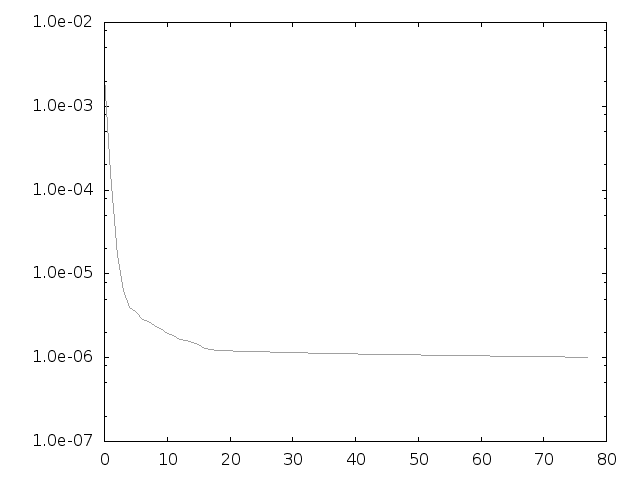
\includegraphics[width=0.45\textwidth]{results/reverse_engineering_LinearNonLinearTransform_N=8/costs} &
    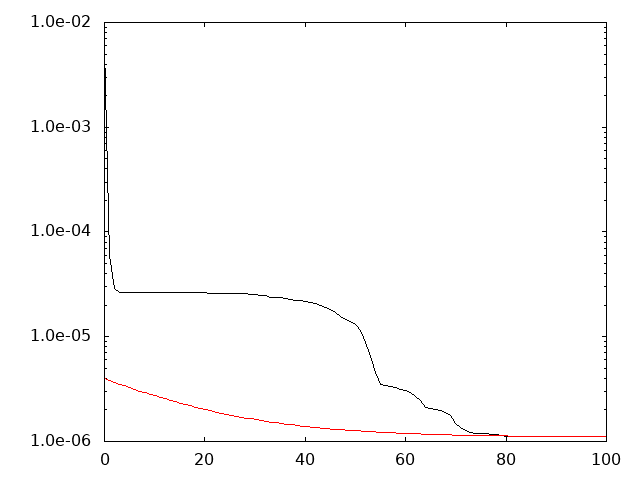
\includegraphics[width=0.45\textwidth]{results/reverse_engineering_IntegrateAndFireTransform_N=8/costs}\\
  \end{tabular}\end{center}
  \caption{Two examples of criterion decay, here for (Left) a {\tt LinearNonLinearTransform} and (Right) {\tt IntegrateAndFireTransform}, with $N=8$, in log-coordinates. The left curve is a ``standard'' curve with a strong decay and then a slow improve of precision. The right curve corresponds to a more erratic behavior with a strong decrease due to the 2nd order mechanism, followed by a ``restart'' of the optimization after a 1st order search thanks to the gradient momentum heuristic.}
  \label{criterion-decay-curve}.
\end{figure}

A key point is that the convergence corresponds to an exponential decay profile, and the decay magnitude almost corresponds to the 2nd order adjustment, when the criterion is locally quadratic, while 1st order fall-back mechanism is mainly chosen by the algorithm in the other cases (e.g. concave criterion), again as expected. We only observed that the 2nd order adjustment may generates weights that can, mainly in the linear case, generates divergent sequences. Despite this caveat, the optimization algorithm recovers by reducing the weight variation amplitude, thus re-obtaining convergent simulation.

We also never observed backward tuning numerical explosion of extinction in all experiments, probably because of the numerical conditioning of the equation has been optimized, but this is to expected in larger scale experiments.

\begin{figure}[!ht]
  \begin{center}{\small 
    \begin{tabular}{l|ccccccc|}
Node type & \multicolumn{7}{c}{LinearNonLinearTransform} \\
\hline
Sample index & 1 & 2 & 3 & 4 & 5 & 6 & 7 \\
Number of Iterations & 101 & 4 & 4 & 3 & 4 & 3 & 4 \\
Minimal criterion value & 1.9e-05 & 2.6e-06 & 2.0e-06 & 4.4e-06 & 1.3e-06 & 9.3e-06 & 6.2e-06 \\
\hline
\end{tabular}

  }\end{center}
  \caption{Variability in term of convergence for a {\tt LinearNonLinearTransform}, with $N=8$, for a standard relative cost of $10^{-5}$, when varying the root network input/output sequence and/or the learning network initial weights draw. Some runs may take quite more time if the initial conditions are far from the solution, whereas we always observe convergence.}
  \label{reverse-engineering-variability}
\end{figure}

\subsection*{Using different criterion}

A step further, we consider an approximate reverse-engineering input/output sequence, with either additive noise or some spurious outliers with large errors. We already know that as soon as the dynamic is sufficiently rich, even small errors accumulate and the solution exponentially diverges from the exact one. In such a case, two questions are raised.

On one hand, can a robust criterion ``resist'' to such noise or outliers ? We have tested this by considering both additive noise and outliers as reported in Fig.~\ref{robust-criterion}. And we have compared the use of several criterion, discussed in Appendix~\ref{application}: ${\cal L}^2$ criterion (i.e. least-square), reweighted ${\cal L}^1$ criterion (i.e. unbounded robust criterion), reweighted ${\cal L}^0$ criterion (i.e. unbounded robust criterion), standard ${\cal L}^1$ related criterion, and standard ${\cal L}^0$ biweight criterion. As expected, due to the optimization method that implicitly assumes the criterion to be locally quadratic, reweighted methods outperform usual ones. Furthermore, without any surprise, a ${\cal L}^2$ criterion is well adapted to additive noise, while a ${\cal L}^1$, or even better a ${\cal L}^0$ criterion, is more resistant to outliers (the numerical results related to these observations are not reported here, but the code is available). All together, we just verify that the proposed mechanism behaves as expected in these various situations.

\begin{figure}[!ht]
  \begin{center}{\small 
    \begin{tabular}{l|ccccc|}
 & \multicolumn{5}{c}{Robustness to noise} \\
\hline
Criterion & 2 & 1 & 0 & a & b \\
Number of Iterations & 4 & 3 & 101 & 4 & 15 \\
Minimal criterion value & 7.8e-05 & 2.0e-04 & 1.2e-04 & 4.5e-04 & 4.4e-02 \\
\hline
\end{tabular}
 \\
    ~\\
    \begin{tabular}{l|ccccc|}
 & \multicolumn{5}{c}{Robustness to outliers} \\
\hline
Criterion & 2 & 1 & 0 & a & b \\
Number of Iterations & 101 & 9 & 4 & 6 & 3 \\
Minimal criterion value & 2.1e-03 & 2.8e-03 & 3.8e-03 & 6.3e-03 & 5.6e-02 \\
\hline
\end{tabular}
 \\
  }\end{center}
  \caption{Robust estimation in the presence of (Top) additive normal noise of relative magnitude $\sigma = 0.1$ and (Bottom) outliers with a probability $\pi = 0.05$ and relative magnitude $\sigma = 10$ using a '2' ${\cal L}^2$ criterion, '1' reweighted ${\cal L}^1$ criterion, '0' reweighted ${\cal L}^0$ criterion, 'a' absolute value, 'b' biweight criterion. The quadratic performs better (considering the number of iterations, the final criterion being of the same order of magnitude) in the presence of noise, while robust criterion are must faster in the presence of outliers.}
  \label{robust-criterion}
\end{figure}

On the other hand, if the deterministic output values diverge, does the output statistics also diverges? The assumption is that though the individual values are very different, the statistical observable (e.g., mean, correlation) can be adjusted. We thus have to compare the KL-divergence between the desired and obtained output given the input, as made explicit in Appendix~\ref{stochastic}. In order to perform this test we have considered directly a random output and evaluated if the {\tt KernelObservableEstimator} can be used with the proposed estimation method. This has been verified with a related precision better than $10^{-3}$ considering a LNL unit, and two simple models:
\\ - Taking the input mean of a given channel $\omega_n(t) = x_n(t)$ into account,
\\ - Taking the input auto-correlation of a given channel $\omega_{n,\tau}(t) = x_n(t) \, x_n(t - \tau)$ into account,
\\ this last couple of tests being very preliminary, while it is a perspective of this work to further investigate in this direction.

\subsection*{Sequence generation}

As a final test, let us consider e.g. the Sierpinski sequence\footnote{This corresponds to the \href{https://en.wikipedia.org/wiki/Sierpinski_triangle}{Sierpinski triangle} read from left to right and from top to down in sequence.}, which is deterministic aperiodic, and a function of the $O(\sqrt{t})$ previous samples at time $t$, thus with long term dependency\footnote{The Sierpinski sequence is generated by recurrent equations of the form:
\eqline{\begin{array}{rcll}
x_0(t) &=& -1 + 2 \, (x_1(t) \mbox{ mod } 2) & x_0(t) \in \{-1, 1\} \\
x_1(t) &=& 1 + \delta_{0 < k_t < l_t < t} \, (x_1(t-l_t) + x_1(t-l_t-1) - 1) & \mbox{Pascal triangle sequence}\\
l_t &=& l_{t-1} + \delta_{k_{t-1} = 0} & l_t = O(\sqrt{t})\\
k_t &=& \delta_{k_{t-1} = l_{t-1}} \, (k_{t-1} + 1) & 0 \leq k_t < l_t\\
\end{array}}}.

As discussed in Appendix~\ref{closedforms}, in the general case and without a specific architecture, we need at least $O(\sqrt{T})$ units to generate an unpredictable sequence of length $T$, without mistakes. Here we have tested with AIF and LNL units and obtained the results reported in Fig.~\ref{sequence-generation}. The units have no input, but there is an offset that allows the units to have some spontaneous activity.

\begin{figure}[!ht]
  \begin{center}{\small 
    \begin{tabular}{l|ccccccc|}
Node type & \multicolumn{7}{c}{LinearNonLinearTransform} \\
\hline
Number of units & 2 & 3 & 4 & 5 & 6 & 7 & 8 \\
Sequence length & 6 & 5 & 6 & 5 & 8 & 7 & 8 \\
Number of Iterations & 36 & 2 & 4 & 2 & 18 & 14 & 16 \\
\hline
\end{tabular}
 \\
  }\end{center}
  \caption{Minimal numbers of unit versus sequence length to generate the Sierpinski sequence without any error, for a network of AIF units and the so called binary criterion.}
  \label{sequence-generation}
\end{figure}

\subsection*{Discussion}

These preliminary tests simply demonstrate that the proposed method works, with better performances than 1st order usual estimation methods. The main positive result is that in all cases only one ``output'' unit is observed while hidden units weights are adjusted without any restriction on the connectivity. Exact estimation can be obtained if a solution exists. The second interesting observation is that it applies to a large class of unit types and criteria. 

These results are quite limited. On one hand, due to computer power availability (running on only one machine with no use of GPU), we have only considered tiny network sizes. However, as discussed in the presentation of the method, as being a distributed mechanism, generalization to much larger setup is really feasible, especially because the algorithm ingredients are quite standard. We also can reasonably hope that the good numerical stability will allow the method to scale up on larger networks. On the other hand, we have not proved here that smaller recurrent networks can outperform huge feed-forward deep networks. However, the question could not be raised before, because weight estimation methods were quite limited, which is not the case here.

We thus can propose these first results as a promising track to further revisit how to estimate weights in recurrent networks.
